\chapter{評価}
\label{chap:evaluation}

本論文で実装した End.AN.NF の性能を評価するために,4つの実験を行った.
本章では,3つの計測実験で得られた結果から,提案手法が実用上十分なスループット性能を持っているか,及び実用的なレイテンシに収まっているのかを確認するために Linux に実装されている既存のパケット転送メカニズムと比較し評価する.
このうち2つはスループットについて,もう1つはレイテンシについて焦点を当てたものである.
最初の実験では,パケットサイズに基づくスループットを計測し,2つ目の実験では,netfilter-based アプリケーションにおけるフィルタールール数を増加させた際のスループットの変化を評価した.
3つ目の実験では,異なるパケット転送メカニズムに関連するレイテンシを計測した.
本章では更に,計測用パケットの送信に利用したトラフィックジェネレータ,及び評価の際に考慮したレシーブサイドスケーリングについても解説する.
また,計測時に netfilter-based アプリケーションとして利用した nftables についても同様に解説する.

\section{計測の概要と予想}
\label{sec:eval-prediction}
End.AN.NF の性能を,3つの転送メカニズムと比較する.
比較対象は,End,End.DT4 と H.Encaps の組み合わせ,及び IPv4 である.
IPv4 は Linux のパケットフォワーディング性能におけるベースラインとして参照する.
図~\ref*{fig:hooks}に示すように,End.AN.NF が動作する場合,受信パケットは End と比較して2倍の数のフックポイントを通過する.
したがって,End.AN.NF の性能は End に劣ることが予想される.
一方で,End.AN.NF の性能は End.DT4 と H.Encaps の組み合わせよりも高いと予想される.

SRv6 でカプセル化されたパケットに netfilter のルールを適用する場合,バニラ Linux カーネルでの実用的なアプローチは End.DT4 と H.Encaps の組み合わせである.
本論文執筆現在,Linux のメインラインには章 \ref{sbsection:use-sr-proxy} で示したような End.AS や End.AD などの SR-Proxy は実装されていない.
本論文では,End.AS や End.AD などの SR-Proxy のかわりにバニラの Linux カーネルで動作する End.DT4 と H.Encaps の組み合わせを End.AN.NF の比較対象とする.
図~\ref*{fig:diff} に,End.AN.NF と End.DT4 と H.Encaps の組み合わせの動作の違いを示す.
End.AN.NF も End.DT4 と H.Encaps の組み合わせも,どちらも SRv6 パケットとして受信したパケットの内部を netfilter フックポイントへ通過させることができる.
章~\ref{sbsection:linux-packet-forwarding} で述べたように,End.AN.NF はパケットバッファ内で IP ヘッダを指し示す部分のポインタを操作することで SRH を隠蔽し,内部パケットを netfilter フックポイントへ通過させる.
対して,End.DT4 と H.Encaps の組み合わせでは,End.DT4 が SRH を一度取り外し,netfilter を適用してから再度 H.Encaps でカプセル化を行う.
Linux カーネルのネットワークスタック的には,End.DT4 がデカプセル化を行うと,そのパケットは VRF で受信される.
VRF で受信されたパケットは,一般的なパケットと同様に netfilter を通過する.
そして,そのパケットの宛先アドレスを VRF 上でルックアップすると,経路情報として H.Encaps によって再度カプセル化されるように記述されているため,H.Encaps によってパケットはもう一度カプセル化される.
つまり,End.DT4 と H.Encaps の組み合わせでは End.DT4 によるデカプセル化処理,デカプセル化されたパケットの VRF での受信,H.Encaps によるカプセル化のオーバーヘッドが存在する.
したがって,このオーバーヘッドが性能の低下につながることが予想されるため,End.AN.NF の性能は End.DT4 と H.Encaps の組み合わせよりも優れていると予想できる.

3つの実験はすべて同じ構成,同じ環境で行った.
マシンの構成を,表~\ref*{tbl:machines}に示す.
100Gbps のリンクで直結された2台のマシンを用意した.
2台のマシンは同一仕様で,CPU には Intel(R) Xeon(R) Silver 4310 12コア x2,メモリは 64GB DDR4-2666,NIC には Intel E810 100Gbps を搭載している.
CPU のハイパースレッディング機能は無効に設定した.
1台はトラフィック・ジェネレータとして,もう1台は System Under Test (SUT) として使用する.
トラフィック生成マシンには Ubuntu 22.04 と TRex~\cite{trex} をインストールし,テストトラフィックの生成に使用した.
一方,SUT マシンには End.AN.NF を実装した Linux カーネル 5.15.106 をインストールし,End.AN.NF と,End.AN.NF の SID を設定するために独自に拡張した iproute2 コマンドを実装した.
また,2台のマシン間のリンクには2つの VLAN を設定し,テストトラフィックを送信するためのリンクと End.AN.NF 動作後に送信されるトラフィックが論理的に別のリンクになるようにした.
VLAN は tag 付きで送信し,Linux カーネルのネットワークスタックが tag をほどく.

\begin{figure}[t]
    \centering
    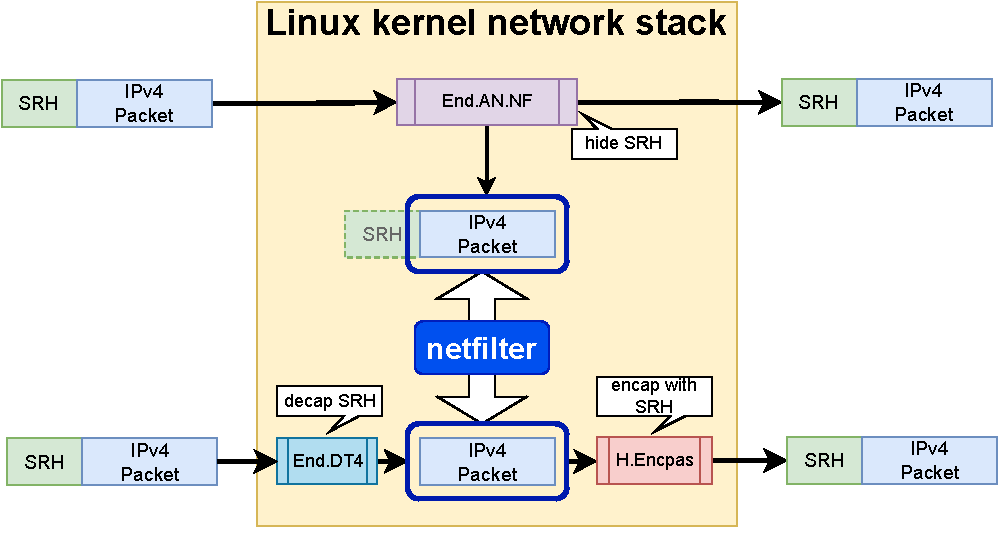
\includegraphics[width=0.95\linewidth]{img/Diff.pdf}
    \caption{End.DT4 と H.Encaps の組み合わせ と End.AN.NF のパケット処理プロセスの差}
    \label{fig:diff}
\end{figure}

\begin{table}[t]
  \centering
  \caption{実験に使用したマシンの構成}
  \label{tbl:machines}
  \begin{tabular}{|c|c|c|cc}
  \cline{1-3}
          & トラフィックジェネレータ                   & System Under Test                  &  &  \\ \cline{1-3}
  カーネル & 5.15.0-79-generic              & customized 5.15.106              &  &  \\ \cline{1-3}
  インストールツール  & TRex v3.03                     & customized iproute2                  &  &  \\ \cline{1-3}
  CPU  & \multicolumn{2}{c|}{Intel(R) Xeon(R) Silver 4310 12コア x2}           &  &  \\ \cline{1-3}
  メモリ  & \multicolumn{2}{c|}{64GB DDR4-2666}                                 &  &  \\ \cline{1-3}
  NIC  & \multicolumn{2}{c|}{Intel E810 100Gbps}                             &  &  \\ \cline{1-3}
  OS   & \multicolumn{2}{c|}{Ubuntu 22.04.2 LTS} &  &  \\ \cline{1-3}
  \end{tabular}
  \end{table}

\section{TRex}
\label{sec:trex}
本論文では,スループット及びレイテンシの計測に TRex を利用した.
TRex は Cisco System によって開発されたトラフィックジェネレータである.
TRex は DPDK~\cite{dpdk} というライブラリを使って開発されている.

DPDK はパケット処理をカーネル空間で行わない.
Linux カーネルにはパケット転送メカニズムが実装されている.
FRR などの Linux ソフトウェアルータ実装は,動作するルーティングプロトコル群がユーザ空間で動作し,NETLINK メッセージを通じて経路情報がカーネルのルーティングテーブルにインストールする.
そして FRR は実際のパケット転送処理を Linux カーネルにまかせている.
対して,図~\ref*{fig:dpdk} に示すように DPDK では NIC で受信したパケットはカーネルをバイパスし,ユーザ空間で操作する DPDK ソフトウェアに渡される.
よって,DPDK のパケット処理性能は Linux カーネルに実装されているパケット処理メカニズムの性能に依存しない.
また,DPDK は CPU を独占する.
DKDP アプリケーションは動作中,指定された CPU へポーリング常にを行う.
これにより,コンテキストスイッチングを抑制して高速な処理を行うことができる.

TRex は柔軟なトラフィック生成が可能である.
最も基本的な使い方は,元となるパケットキャプチャファイルを用意し,トラフィックごとに変更する部分を別途 yaml ファイルで定義するという方法である.
この yaml ファイルには,例えば送信元 IP アドレスや宛先 IP アドレスを定義することができる
TRex はこのファイルの内容に従って,元となるパケットキャプチャファイルの情報を変更し,パケットキャプチャファイルとは別の送信元 IP アドレスや宛先 IP アドレスを持つパケットを生成し,送信することができる.
また,どれだけの時間,単位時間あたりにどれだけのパケットを送出するのかといったことも yaml ファイルに定義できる.

また,パケットキャプチャファイルを利用する方法以外にも,Python スクリプトを使ってパケットを生成し送出することができる.
\texttt{trex\_stl\_lib.api} という Python ライブラリに様々な API が提供されている
このライブラリには SRv6 パケットを生成する関数も提供されており,本論文では,この Python スクリプトを使ってトラフィックを生成する手法でパケットを生成し計測した.
本論文での計測実験では,IPv4 パケットを特定の SRH でカプセル化する.
一部の実験時にはレシーブサイドスケーリングの仕組みを効率的に使うため,カプセル化する IPv4 パケットの送信先アドレスをインクリメントした.
TRex はこのように,SRv6 のパケットの生成,及び内部パケット情報の操作も可能である.

\begin{figure}[t]
    \centering
    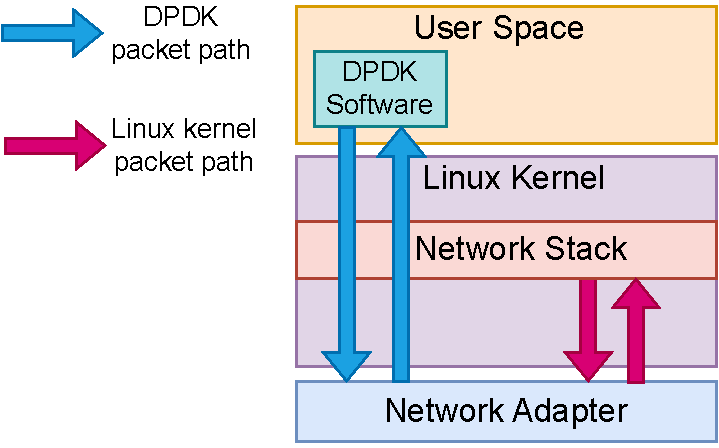
\includegraphics[width=0.95\linewidth]{img/DPDK.pdf}
    \caption{DPDK アプリケーションの動作概要}
    \label{fig:dpdk}
\end{figure}

\section{レシーブサイドスケーリング (RSS)}
\label{sec:rss}
レシーブサイドスケーリング (RSS) とは,マルチコアプロセッサを搭載したシステムにおいて,パケットの受信処理を複数の CPU コアに分散させる技術である.
これにより,CPUコアの負荷が均等に分散され,スループットの向上が期待できる.
図~\ref*{fig:rss} に示すように,RSS では受信したパケットからハッシュを計算し,その値をもとに RX キューを分散させる.
RSS の実装は NIC のドライバに依存する.
ハッシュの計算アルゴリズムは NIC のドライバの実装によって異なる上,パケットのどの部分からハッシュを計算するかも異なる.

一般的な SRv6 ネットワークではパケットを SRH でカプセル化するノードの数は限られるため,ドライバの実装が SRH の送信元及び宛先アドレスをキーにしてハッシュを計算する手法を取っている場合,ハッシュの値が偏ってしまう.
本論文では,計測対象のパケットは SRv6 パケットである.
SRv6 パケットは SRH でカプセル化されている.
一般的な SRv6 パケットの送信元アドレスにはパケットを SRH でカプセル化するノードのループバックアドレスが割り当てられ,宛先アドレスには次の SRv6 ノードの SID が割り当てられる.
つまり,SRv6 ビヘイビアを実行するノードが受け取るパケットの送信元アドレスは SRH でカプセル化するノードのループバックアドレスであり,宛先アドレスは自分自身の SID である.

本計測では,SRv6 パケットに対して RSS を有効化する必要がある際は,SRH でカプセル化された内部パケットの宛先アドレスを変更する.
本計測で利用した環境では,NIC として E810 を利用した.
実際にパケットキャプチャをして検証した結果,E810 では SRv6 パケットに対して RSS を適用するためには内部パケットの宛先アドレスを変更すれば良いことがわかった.
SRH でカプセル化された内部パケットの宛先アドレスは,そのパケットの送信元が実際に通信するエンドノードのアドレスである.
したがって,実運用上,SRH でカプセル化された内部パケットの宛先アドレスがバラバラになることは自然なシナリオである.


\begin{figure}[t]
    \centering
    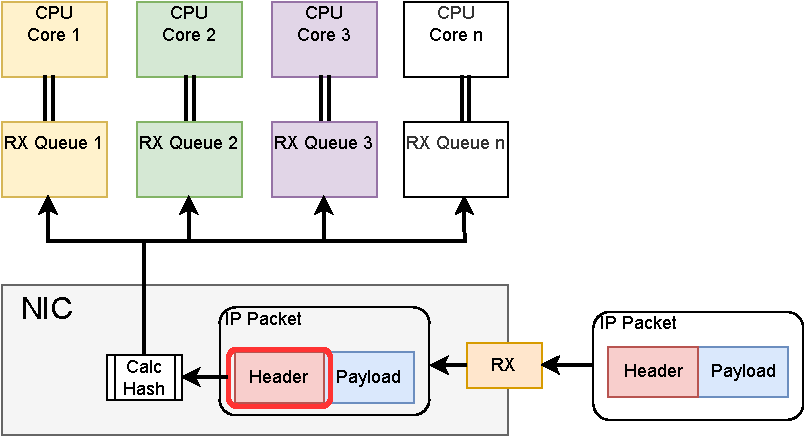
\includegraphics[width=0.95\linewidth]{img/RSS.pdf}
    \caption{レシーブサイドスケーリングの動作概要}
    \label{fig:rss}
\end{figure}

\section{パケットサイズ毎のスループット性能}
\label{sec:eval.thru-size}
End.AN.NF,End,IPv4,及び End.DT4 と H.Encaps の組み合わせについて,パケットサイズを増加させながらスループットを測定した.
この実験により,各パケット転送メカニズムにおけるパケットサイズによるスループットの変化が明らかになった.
この実験では,netfilter フックポイント通過時に適用されるルールはからの状態で実施した.
よって,netfilter のフックポイントは通過するものの,実際にパケットにフィルタやマングルルールが適用されることはない.
End.AN.NF の,End に対するスループットの低下,及び End.DT4 と H.Encaps の組み合わせに対する性能の向上を評価した.

\subsection{計測内容}
\label{ssec:thru-size.summary}
トラフィック生成マシンで TRex によって生成されたトラフィックを,最小パケット長 126 バイトから最大パケット長 1518 バイトまでパケットサイズを変化させ,SUT マシンに送信した.
測定時のパケット長は次のように計算した: $l=174n+126$.
ここで $l$ はパケット長,$n$ は測定回数である.
$n=0$ から $n=10$ まで,合計10回の測定を行った.

最小パケット長として 126 バイトを選択した理由は,SID リストの長さが 2 である際のタグ付き VLAN を持つ UDP パケットの最小長が 126 バイトだからである.
End.AN.NF は,パケットの segleft をデクリメントするため,SID リスト長は少なくとも 2 である必要がある.
これは SID リストの長さが 1 の場合,segleft は 0 から始まり,End.AN.NF でデクリメントすると負の値になってしまうからである.
一方,End.DT4 は,segleft が 0 であることを必要とする.
End.DT4 は SRv6 ネットワークの終点で SRH をでカプセル化するビヘイビアである.
つまり,End.DT4 が動作するのは SID リストによって指定された最後のノードであるため,segleft はそれ以上デクリメントできない 0 である必要がある.
そこで,End.DT4 と H.Encaps の組み合わせの測定では,TRex は SID リスト長が 2 のパケットを生成し,segleft を 0 に設定した.
また,レシーブサイドスケーリング (RSS) の仕組みを効果的に使用するため,TRex でパケットを生成する歳に内側の IPv4 パケットの宛先アドレスと送信元アドレスの両方をインクリメントした.
IPv4 パケットの計測の際は,SRv6 パケット長に合わせて UDP ペイロードにダミーデータを埋め込み,最小パケット長が 126 バイトから始まるようにした.
End.DT4 と H.Encaps の組み合わせの計測と同様,RSS を効果的に活用するため,パケット生成時に宛先アドレスと送信元アドレスをインクリメントした.
最大パケット長については,タグ付き VLAN ヘッダを含むイーサフレームの最大サイズが 1518 バイトであることから,今回の測定ではパケットサイズの上限を 1518 バイトに設定した.

\subsection{評価}
\label{ssec:thru-size.eval}
図~\ref{fig:size-thru} に,この実験の結果を示す.
End.AN.NF のスループットは,すべてのパケット長において End と比較して 6\% 以上の低下は見られない.
パケット長が 1518 バイトのとき,End.AN.NF は End と比べた際のスループットの低下が最も少なく,その低下は約 1.7\% である.
対して,パケット長が 478 バイトのとき,End と比較した際の End.AN.NF のスループットの低下は最も大きく,その低下は 約5.6\% である.
パケット長とスループットには相関がなく,大きな変動が見られた.
このスループットの低下は,End.AN.NF のパケットが End のパケットに比べて2倍の netfilter のフックポイントを通過することが原因として挙げられる.
ただし,そのスループット低下のレベルは許容範囲内に留まっている.

End.AN.NF のスループットを End.DT4 と H.Encaps の組み合わせと比較した場合,End.AN.NF は予想通り,パケット長に関係なく一貫して優れた性能を示している.
具体的には,End.AN.NF は End.DT4 と H.Encaps の組み合わせよりも,最大で 26.7\% 高いスループットを達成している.
グラフから,End.AN.NF と End.DT4 と H.Encaps の組み合わせとの間のスループットの差はパケット長の影響を受けていることが読み取れる.
短いパケットでは相対的な性能格差が大きくなり,長いパケットではその差は縮まる.
パケットサイズが小さくなるにつれて,1秒あたりのパケット転送レート (pps) は増加する.
結果として,パケットサイズが小さいほど,パケット転送のオーバーヘッドが顕著になる.

\begin{figure}[t]
    \centering
    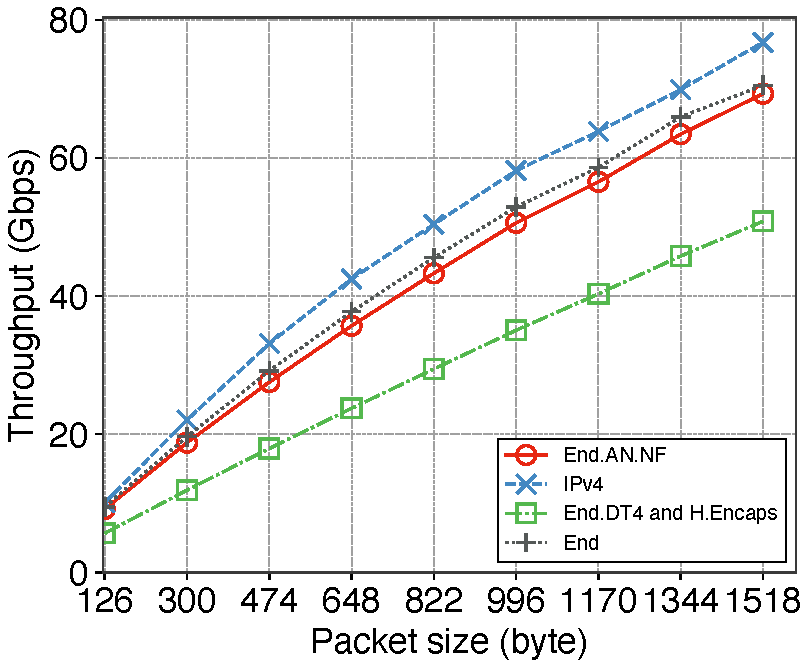
\includegraphics[width=0.95\linewidth]{img/size-throughput.pdf}
    \caption{SRv6 End ビヘイビア毎,及び IPv4 のスループット}
    \label{fig:size-thru}
\end{figure}


\section{netfilter にインストールされたルール毎のスループット}
\label{sec:eval.thru-chains}
次に,End.AN.NF,IPv4,および End.DT4 と H.Encaps の組み合わせについて,netfilter にインストールするフィルタールールの数を変更しながらスループットを測定した.
フィルタールールのインストールには,netfilter-based アプリケーションとして nftables を使用した.
nftables では,ルールはチェインの集合として表現され,チェインにはベースチェインとレギュラーチェインの2種類がある.
nftables は,他のチェインがレギュラーチェインを参照している場合のみ,レギュラーチェインを使用する.
実験では,チェインの種類ごとにカウントを増やしながらスループットを測定した.
パケット転送メカニズムに関わらず,フィルタールールの追加によりスループットが低下することが予想される.
この実験は,フィルタールールによる各パケット転送メカニズムのスループット低下の特徴を明らかにすることを目的とする.

\subsection{nftables}
\label{ssec:thru-chains.nftables}
本セクションでは,nftables について解説する.
nftables 公式 wiki~\cite{about-nftables} によると,nftables とはモダンな Linux カーネル向けのパケット分類フレームワークだという.
nftables を使うと,パケットのフィルタリングや NAT,NAPT やその他のパケットマングリングを適用することができる.
対象は自身宛のパケットだけでなく,自信がトランジットとなる通信や自身が送出するパケットなど様々な種類のパケットに対してルールを適用できる.
nftables は iptables の後継フレームワークであり,iptables の抱えるいくつかの問題点を改善したフレームワークである.
例えば,nftables のルール定義文法は iptables のルール定義文法に比べて,より構造化されている.
自身の 80 番ポートに対する tcp 通信を拒否する,というフィルタールールを定義する設定ファイルを,nftables と iptables それぞれについて確認する.
nftables 向けの定義ファイルをソースコード~\ref*{nft-filter-rule} に,iptables 向けの定義ファイルをソースコード~\ref*{ipt-filter-rule} に示す.

nftables では,ルールセットの塊を \texttt{table} という単位で管理する.
この \texttt{table} には予約されている特定の語句や記号を除き,任意の名前で定義することができる.
テーブルを定義する際は,\texttt{table} \textit{family} \textit{table\_name} のフォーマットで記述する.
\textit{family} には,IPv4 パケットを対象とするテーブルには \texttt{ip} が,IPv6 パケットが対象であれば \texttt{ip6} が,両方が対象であれば  \texttt{inet} が入る.
対して,iptables は IPv4 と IPv6 のルールを同じ枠組みで書くことができない.
iptables は IPv4 向けのユーティリティであり,IPv6 には ip6tables を利用する必要がある.

ソースコード~\ref*{nft-filter-rule} 2 行目では,\texttt{deny8080} という名前でチェインが定義されている
チェインはテーブルの中に任意に数定義することができ,そのフォーマットは \texttt{chain} \textit{chain\_name} である.
ソースコード~\ref*{nft-filter-rule} 3 行目では,ネットフィルターフックポイントに登録する際に必要な情報が定義されている.
\texttt{type filter} はチェインのルールがフィルターであることを表している.
\texttt{hook input priority filter} は,「フィルタールールのデフォルトの優先度で,netfilter の input フックポイントに対象のチェーンを登録する」ということを示している.
図~\ref{fig:nf-hooks} で示したように,input フックポイントは通信のエンドポイントが自分自身である際に通過するフックポイントである.
ソースコード~\ref*{nft-filter-rule} 4 行目では,実際のルールが定義されている.
通信プロトコルが tcp であり,宛先ポートが 8080 番であればドロップされる.

対して iptables では,実質的なルールの定義はソースコード~\ref*{nft-filter-rule} の 1 行目及び 2 行目だけである.
\texttt{*filter} は 対象がフィルタールールであることを示し,\texttt{-A INPUT} でルールを input フックポイントに設定することを示し,以降は宛先ポートが 8080 番の tcp 通信を拒否するように書かれている.
iptables では,ルールの定義をトランザクションとして管理するため,定義しただけでは変更が反映せれず,\texttt{COMMIT} キーワードで明示的に変更の反映を示す必要がある.

nftables のルール定義は,iptables のルール定義に比べて記述量が多くなる傾向がある.
一方で,nftables のルール定義は iptables のルール定義に比べて宣言的で構造化されているため,ルール数が増えたときに人間が読んで理解しやすいフォーマットになっている.
2 つのルールの定義方法は違うが,現在の Linux では,iptables でルールを定義すると内部的には nftables のルールに変換される.
これは nftables の方が従来の iptables よりも性能面でのアドバンテージが大きいからである.

チェインにはベースチェインとレギュラーチェインの 2 種類が存在し,nftables はひとつひとつのルールをチェインという単位で管理する.
ベースチェインとはソースコード~\ref*{nft-chain} の 10 行目から 14 行目までで定義されている \texttt{filter\_rule} チェインを指す.
ベースチェインを宣言すると,そのチェインに対応するルールが netfilter フックポイントに設定されるため,ソースコード~\ref*{nft-chain} の\texttt{filter\_rule} チェイン内のルールは,自身が IPv4 パケットの転送動作をする際は必ず適用される.
一方で,ソースコード~\ref*{nft-chain} 中の \texttt{remote\_access} チェインと \texttt{rate\_limit} チェインはレギュラーチェインと呼ばれるチェインである.
レギュラーチェインには,ソースコード~\ref*{nft-chain} 11 行目のようなルールのタイプと netfilter フックポイントを指定する項目がない.
レギュラーチェインは,定義しただけではどの netfilter フックポイントにも結び付けられず,実行されない.
レギュラーチェインは他のチェインからの参照によってのみ実行される.
例えば,ソースコード~\ref*{nft-chain} の 12 行目,13 行目では,パケットバッファのマークフィールドに特定の値が値が代入されていることを条件とし,\texttt{goto} キーワードを使って指定したチェインを呼び出している.
このように,レギュラーチェインは \texttt{goto} キーワードで呼び出されて初めて実行される.
ソースコード~\ref*{nft-chain} ではベースチェインからレギュラーチェインを呼び出しているが,レギュラーチェインはその処理の中で別のレギュラーチェインを呼び出すこともできる.
つまり,レギュラーチェインは定義しただけでは実行されず,他のベースチェインまたはレギュラーチェインから参照されて初めて実行される種類のチェインである.

% \begin{lstlisting}[caption=Definition of simple filter rule for nftables,label=nft-filter-rule]
\begin{lstlisting}[caption=nftables におけるシンプルなフィルタルールの定義例,label=nft-filter-rule]
table ip filter_sample {
  chain deny8080 {
    type filter hook input priority filter;
    tcp dport 8080 drop
  }
}
\end{lstlisting}

% \begin{lstlisting}[caption=Definition of simple filter rule for iptables,label=ipt-filter-rule]
\begin{lstlisting}[caption=iptables におけるシンプルなフィルタルールの定義例,label=ipt-filter-rule]
*filter
-A INPUT -p tcp --dport 80 -j DROP
COMMIT
\end{lstlisting}

% \begin{lstlisting}[caption=An example of a definition: regular chain and base chain,label=nft-chain]
\begin{lstlisting}[caption=nftables におけるレギュラーチェインとベースチェインを利用したルールの定義例,label=nft-chain]
table ip fw01 {
  chain remote_access {
    tcp dport ssh drop
    tcp dport telnet drop
    accept
  }
  chain rate_limit {
    ip protocol icmp icmp type echo-request limit rate over 1/second drop
  }
  chain filter_rule {
    type filter hook forward priority filter;
    meta mark 0x1111 goto remote_access
    meta mark 0x2222 goto rate_limit
  }
}
\end{lstlisting}

\subsection{計測内容}
\label{ssec:thru-chains.summary}
トラフィック生成マシンで TRex が生成したトラフィックを SUT マシンに送信した.
この測定では,パケット長を一貫して 126 バイトに設定した.
パケット長を 126 バイトに設定した理由はセクション~\ref{ssec:thru-size.summary} で説明したものと同じで,SID リスト長が 2 の場合のタグ付き VLAN の UDP パケットの最小長が 126 バイトだからである.

\subsection{評価}
\label{ssec:thru-chains.eval}
図~\ref{fig:rule-thru}は,ベースチェインのルール毎のスループットを示している.
全てのチェインルールがベースチェインのみで構成されるこれらのチェインルールは,nftables のチェインルールの定義の中でも最も性能の出ないルール定義の1つである.
この測定では,netfilter のフォワードフックポイントにフィルタールールを設定した.
netfilter は 1 つのフックポイントに複数のルールを設置できる.
実験を通して,このフックポイントで適用される同一のカスケードルールの数を増加させた.
すべてのパケット転送メカニズムにおいて,スループットはルール数の増加と共に低下する.
ルール数が増加するにつれて,3 つのパケット転送メカニズムすべてのスループットは約 0.4 Mbps に収束することがわかった.
End.AN.NF と IPv4 のスループットを比較すると,スループット低下における顕著な特性の違いは見られず,End.AN.NF は IPv4 に対して大きく劣るスループット低下特性を示さない.
一貫して,End.AN.NF は End.DT4 と H.Encaps の組み合わせのスループットを上回る.
しかし,このスループットの差はルール数が増えるにつれて縮小し,128 ルールではわずか 9\% の差まで減少した.
これは,ルール数が増加するに従ってパケット転送にけるオーバーヘッドの割合が変化したからだと考えられる.
ルール数が少ないうちはパケットのカプセル化とデカプセル化にかかるオーバーヘッドが割合として大きく,ルール数が増えるに従って,netfilter の処理にかかるオーバヘッドの割合が増える.
netfilter の処理にかかるオーバヘッドは End.AN.NF と End.DT4 と H.Encaps の組み合わせで同じであるため,スループットの差が縮まったと考えられる.
結果として,レギュラーチェインのルール数が増加するにつれて,End.AN.NF の End.DT4 と H.Encaps の組み合わせに対する優位性は低下すると言える.


図~\ref{fig:reg-thru}は,ベースチェインのルール数毎のスループットを示している.
注目すべき点は,ルール数を増加させてもスループットの低下が認めれず,かつ End.AN.NF が一貫して End.DT4 と H.Encaps の組み合わせを上回っていることである.
レギュラーチェインのフィルタールールは,ベースチェインで測定した際と同じ構成である.
通過するパケットをすべてアクセプトするルールが定義されており,一度受け入れるルールが適用されたあとも,事前に決めた回数同じ内容のルールが適用され続ける.
しかし,レギュラーチェインのみから成るこのようなルール構成では,定義されたレギュラーチェインが他のチェインから参照されていないため,実際にはルールがパケットへ適用されることはない.
その結果,パケットが netfilter のフックポイントを通過する際に実際に適用されるルールの数は変わらない.

どちらの実験でも,End.AN.NF のスループットは一貫して End.DT4 と H.Encaps を組み合わせる手法を上回った.
また,End.AN.NF のスループットは IPv4 には一貫して劣るものの,End.AN.NF のスループット低下特性は IPv4 と似ており,End.AN.NF のスループット性能は実用上問題ないことがわかった.

\begin{figure}[t]
  \centering
  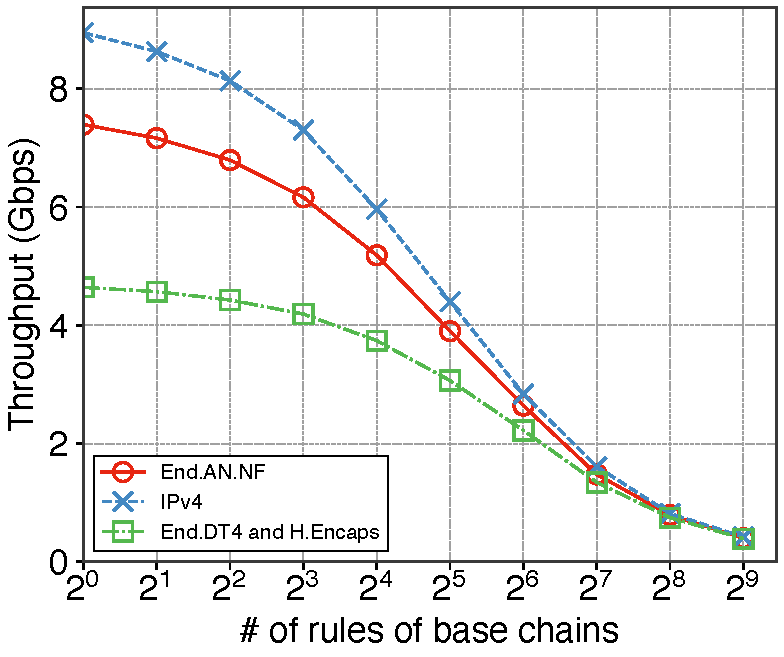
\includegraphics[width=0.95\linewidth]{img/rule-throughput.pdf}
  % \caption{Throughput per number of rules of base chains}
  \caption{ベースチェインのルールごとのスループットの}
  \label{fig:rule-thru}
\end{figure}

\begin{figure}[t]
  \centering
  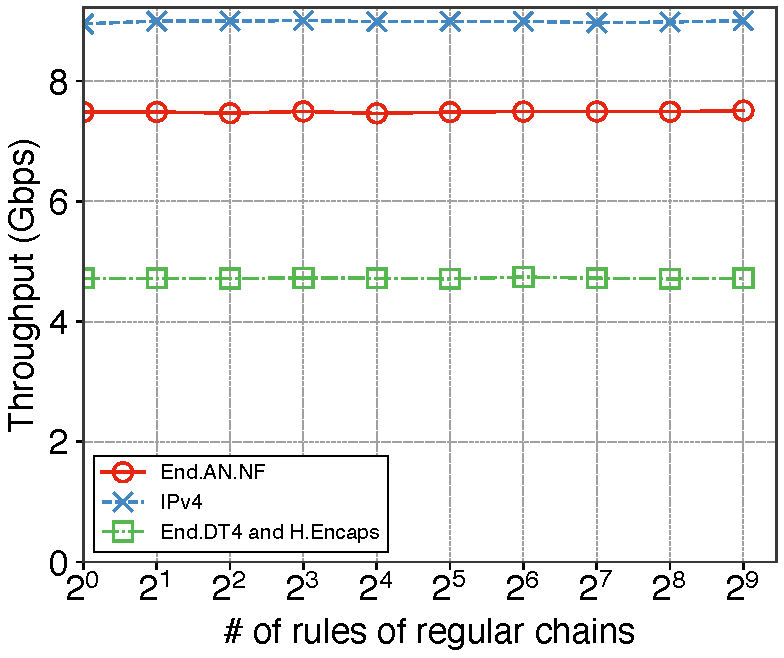
\includegraphics[width=0.95\linewidth]{img/regular-throughput.pdf}
  % \caption{Throughput per number of rules of regular chains}
  \caption{レギュラーチェインのルールごとのスループットの}
  \label{fig:reg-thru}
\end{figure}

\section{レイテンシ}
\label{sec:eval.rtt}
スループットと同様に End.AN.NF,End,IPv4,及び End.DT4 と H.Encaps の組み合わせについて,レイテンシを測定した.
この計測では特に,End.DT4 と H.Encaps の組み合わせと比較して,End.AN.NF のレイテンシがどれだけ改善されたのか評価することを目的としている.
この評価では,ベースラインとして IPv4 のレイテンシを用いた.

\subsection{計測内容}
\label{ssec:rtt.summary}
スループットと同様に,計測には TRex を使用し,パケット転送のレイテンシを測定した.
TRex はパケットの送受信時間間隔をマイクロ秒単位で測ることが可能である.
今回の測定は,パケット長を 142 バイトに設定した.
142 バイトの内訳について,先頭 126 バイトはセクション~\ref{ssec:thru-size.summary} で説明した通りで,End.AN.NF がの動作要件を満たす最小のパケットとして必要だからである.
追加の 16 バイトは,TRex がよるレイテンシを測定する際に利用するメタデータの埋め込みに使用される.
実験中,トラフィック生成マシンは SUT に対して毎秒 10000 個のパケットを10秒間送信した.
今回のレイテンシ測定では,RSS を無効化するために送信元アドレスと宛先アドレスを変更しなかった.
なぜなら,この規模の pps で RSS を使用してパケットを処理する CPU コアを分散させてしまうと,かえってレイテンシが悪化し,余分なジッタが発生することがあるからである.

\subsection{評価}
\label{ssec:rtt.eval}
計測結果を図\ref{fig:rtt} に示す.
これらのグラフの各データポイントは,100000 回のレイテンシ測定の平均値を表している.
End.AN.NF,End,IPv4 のレイテンシはどれも 16.0 マイクロ秒である.
対照的に,End.DT4 と H.Encaps の組み合わせは 19.0 マイクロ秒のレイテンシである.
マイクロ秒単位での測定では,End.AN.NF のレイテンシは End と IPv4 のレイテンシと一致し,End.DT4 と H.Encaps の組み合わせのレイテンシよりも約 15.8\% 高速であることが分かる.
よって,End.AN.NF のレイテンシはマイクロ秒単位であれば IPv4 及び End と同じであり,End.DT4 と H.Encaps の組み合わせのレイテンシよりも約 15.8\% 遅延が改善された.

\begin{figure}[t]
  \centering
  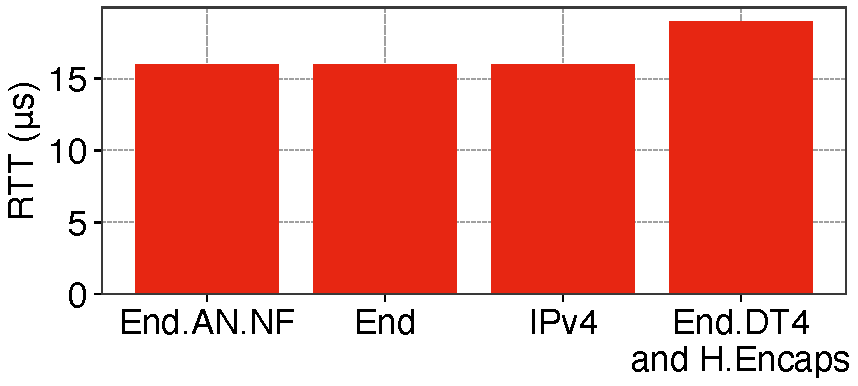
\includegraphics[width=0.95\linewidth]{img/latency.pdf}
  % \caption{Latency per SRv6 End behaviors and IPv4}
  \caption{SRv6 End ビヘイビア毎,及び IPv4 のレイテンシ}
  \label{fig:rtt}
\end{figure}